\section{Iteration \#2 -- Pyramid Tree and the Limitations with Hash-Based Approaches}

TODO
\begin{itemize}
	\item TODO
\end{itemize}

\subsection{Pseudo-Pyramid Tree Optimisations}

The Pseudo-Pyramid Tree performed better than Sequential Scan for point queries in high-dimensional data, up until a certain number of dimensions were reached. This section discusses the different optimisations and variants of this structure that were developed to increase its speed further and make it usable with a higher number of dimensions.

\subsubsection{Accelerating Hash Function}

It was shown in the last iteration that the Pseudo-Pyramid tree eventually becomes slower than Sequential Scan as $d$ increases. Since the plots showed the increase in the Pseudo-Pyramid Tree's execution time is roughly quadratic, and the structure spend most of that time in the $O(d^2)$ hashing function (Equation \ref{eq:pseudo-pyramid-hash}), it follows that speeding up the hashing function would provide large speed gains.

The existing point hashing function takes $O(d^2)$ time because of the inner loop that computes $\prod_{j=0}^{i}{\lbrack m_j \rbrack}$. If $m$ is changed during the structure's lifetime. otherwise the hash value of a point could change and stored points can become inaccessible. Therefore, $m$ is constant and the hashing function can computed in $O(d)$ time by \textit{pre-computing} $\prod_{j=0}^{i}{\lbrack m_j \rbrack}$. This pre-computation happens when the Pseudo-Pyramid tree is initialised. The new hashing function is given in Equation \ref{eq:new-pseudo-pyramid-hash}.

\begin{multline}\\
	h(p) = \sum_{i = 0}^{d} { \lbrack \texttt{toInt}( h_i(p) \times m_i ) \times M_i \rbrack } \\
	\text{where } M_i = \prod_{j=0}^{i}{\lbrack m_j \rbrack} \;\;\; \text{for} \; 0 \leq i \leq d \\
	\label{eq:new-pseudo-pyramid-hash}
\end{multline}

Table \ref{tab:new-pseudo-pyramid-hash} shows operation execution time of the Batch Pyramid Tree using the original $O(d^2)$ hashing function and the new $O(d)$ function. The tes used the Insert-Query-Remove operation list on the uniform synthetic dataset with 200 dimensions. Figure \ref{fig:new-pseudo-pyramid-hash} plots the performance of the Pseudo-Pyramid tree with both hash functions alongside Sequential Scan, showing execution time against dimensionality. From the plot, it is clear that the new hashing function provides superior speed; the Pseudo-Pyramid Tree is now significantly faster than Sequential Scan, even for dimensions as high as 200.

\begin{table}
	\centering
	\begin{tabular}{|l|l|l|}
		\hline
		\textbf{Operation} & \textbf{$O(d^2)$ Function} & \textbf{$O(d)$ Function} \\
		\hline
		\textbf{Insert} & 1.46412 & 0.0112199 \\
		\textbf{Delete} & 0.730777 & 0.00625336 \\
		\textbf{Point Query} & 0.731469 & 0.0076015 \\
		\hline
	\end{tabular}
	\caption{Total Execution Time (in Seconds) of Batch Pseudo-Pyramid Tree Using $O(d^2)$ and $O(d)$ Hash Function (200D Randomly Uniform Dataset, 10,000 operations each)}
	\label{tab:new-pseudo-pyramid-hash}
\end{table}

\begin{figure}
	\centering
	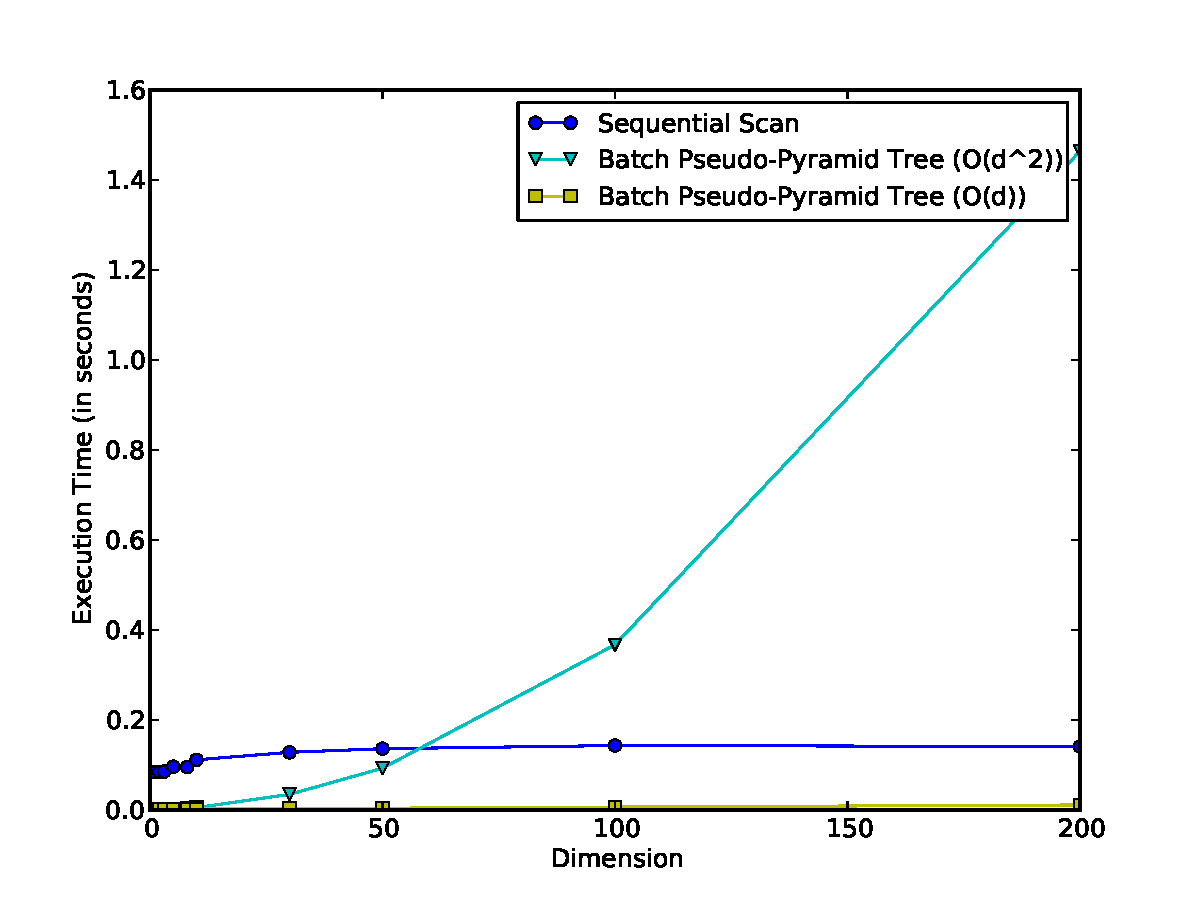
\includegraphics[scale=0.5]{figures/performance_analysis/iteration_2/new_pseudo-pyramid_hash_performance.pdf}
	\caption{\texttt{insert} Performance on Random Uniformly Distributed Datasets of Varying Dimensions}
	\label{fig:new-pseudo-pyramid-hash}
\end{figure}

\subsubsection{Bucket Pseudo-Pyramid Tree}

The Bucket Pseudo-Pyramid Tree implementation does not use a single array to store the points. Instead of buckets containing an array of point indices, it has an array of actual points. No clenaup procedure is necessary because the memory for a point is released immediately afer it's removed, by simply erasing it from the corresponding bucket's array. The goal of this is to increase \textbf{cache coherency} when searhcing a bucket, since the point array can be searched sequentially. The index-based variants cause random accesses in the single point array (causing more cache misses) since a bucket's store indices may point to distant parts of the point array, which may become very large.

% TODO: further explanation of cache misses?

Array deletion is a $O(n)$ operation since the case where a single bucket stores all $n$ points is possible, making \texttt{delete} $O(n)$ in the worst case. Since the order the points are stored in a bucket do not matter, the C++ \textit{erase-remove} idiom has been used to delete elements from the bucket arrays, which swaps the element to delete with the last element in the array, removing the desired element when it's at the end of the array. This prevents the required $O(n)$ shift operation which tightly pack the elements after a deletion.

\paragraph{\textbf{NOTE: }} From this point in the document onwards, all \texttt{std::vector} deletions where order does not matter will be performed using the erase-remove idiom.

\subsubsection{Splay Pseudo-Pyramid Tree}

Unlile the other implementations, the Splay Pseudo-Pyramid Tree does not use a hash map as the underyling one-dimensional index structure, but a splay tree. The splay tree is a self-adjusting variant of the binary search tree that uses a \textit{splaying} operation (a heuristic) to allow faster access to recently accessed elements. \cite{splay-tree}. The splaying operation achieves this by performing a series of tree rotations that move a given node up to the root of the tree. Through amortised analysis and empirical experiments, it has been shown splay trees can be more efficient than standard binary trees for a series of non-random operations \cite{splay-tree}, despite the asymptotic worst case bound being worse than binary search trees.

TODO: more detail about the splay tree, including in-depth algorithms??

Nodes in the Splay Pseudo-Pyramid Tree correspond to individual buckets in the Bucket Pseudo-Pyramid Tree, meaning each node can store multiple points. Since the splay tree is implemented as a collection of heap-allocated nodes with pointers to link them, deletions are cheap as a low amount of memory needs to be de-allocated per \texttt{delete} operation. The aim is that this, combined with the self-adjusting nature of the splay tree, will produce a Pseudo-Pyramid Tree implementation that is more efficient for non-random operations used in real applications.

\subsubsection {Best Pseudo-Pyramid Tree Variant}

All variants of the Pseudo-Pyramid Tree hash $d$-dimensional points to a one-dimensional value, which is used as a key to search for a given point in a one-dimensional structure. What varies is how points are deleted and which underyling one-dimensional structure is used. The Defragmented Pseudo-Pyramid Tree is clearly inferior to the Rebuild Pseudo-Pyramid Tree from the last iteration and the Batch Pseudo-Pyramid Tree never releases memory after points are removed. For dynamic data which changes frequently, this may cause the machine to run out of memory. As such, both of these structures will not be explored further.

% TODO: create new plot
\begin{wrapfigure}[12]{r}{0.5\textwidth}
	\vspace{-40pt}
	\begin{center}
		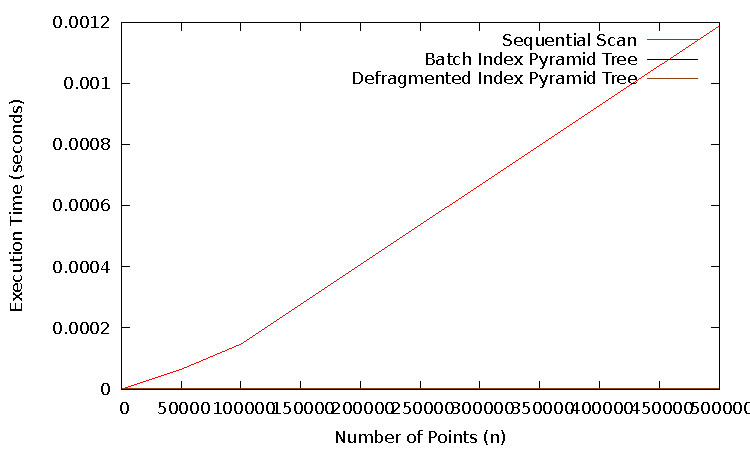
\includegraphics[scale=0.5]{figures/performance_analysis/iteration_1/all_pquery_sizevary_average.pdf}
	\end{center}
	\vspace{-20pt}
	\caption{Total Execution Time (in Seconds) of \texttt{delete} Operation for Different Sample Sizes of Astrophysics Dataset}
	\label{fig:perf2-astrophysics-delete}
\end{wrapfigure}

The Rebuild Pseudo-Pyramid Tree, Bucket Pyramid-Tree and the Splay Pseudo-Pyramid Tree were timed with the full collection of synthetic and real datasets. The results were consistent throughout the different datasets. For brevity, only the times for the astrophysics dataset with the Insert-Query-Delete operation list will be provided. Table \ref{tab:perf2-astrophysic} shows the total execution times of each structure operation and Figure \ref{fig:perf2-astrophysics-delete} shows execution time of the \texttt{delete} operation as the number of points are increased.

The results show that storing separate pint arrays for each bucket drastically reduces the speed of \texttt{delete} operations, with the Rebuuild Pseudo-Pyramid tree being slowest. The differences in speed between the bucket and splay variants is small, but the Bucket Pseudo-Pyramid Tree outperforms the Splay Tree with most datasets. With severely skewed synthetic data, the splay variant is \texttt{slightly} faster, but the speed increase is neglible. This could be an indication that self-adjusting structures are useful for heavily skewed data however, highlighting an area for further study. Based on these results, it was decided that any future variants of the tree will be based on the Bucket Pseudo-Pyramid Tree.

\begin{table}
	\centering
	\begin{tabular}{|r|l|l|l|l|}
		\hline
		\textbf{Structure} & \textbf{Operation List} & $n = 10,000$ & $n = 100,000$ & $n = 500,000$ \\
		\hline
		\multirow{ 4}{*}{\textbf{Rebuild Pseudo-Pyramid Tree}} & \textbf{Insert} & 0.0698843 & 5.99686 & 156.281 \\
		 & \textbf{Delete} & 0.481668 & 59.3513 & 1328.2 \\
		 & \textbf{Point Queries} & 0.0656809 & 5.96501 & 158.955 \\
		\hline
		\multirow{ 4}{*}{\textbf{Bucket Pseudo-Pyramid Tree}} & \textbf{Insert} & 0.0508634 & 4.5737 & 101.581 \\
		 & \textbf{Delete} & 0.318228 & 29.4124 & 672.372 \\
		 & \textbf{Point Queries} & 0.0495212 & 4.43291 & 96.1636 \\
		\hline
		\multirow{ 4}{*}{\textbf{Splay Pseudo-Pyramid Tree}} & \textbf{Insert} & 0.0509274 & 4.64242 & 101.245 \\
		 & \textbf{Delete} & 0.318251 & 29.6108 & 675.695 \\
		 & \textbf{Point Queries} & 0.0507686 & 4.59311 & 99.1579 \\
		\hline
	\end{tabular}
	\caption{Total Execution Time (in Seconds) for Different Sample Sizes of Astrophysics Dataset using the Insert-Query-Delete Operation List}
	\label{tab:perf2-astrophysics}
\end{table}

\subsubsection{Impact of Bucket Size and Boundary Distance Hashing}

TODO: state how even though it's faster than sequential scan -- it's still only about 4/5 times faster than $O(n)$ sequential scan! why??????? BUCKET SIZE! THIS IS THE CORE FACTOR IN PERFORMANCE WITH THESE METHODS!

TODO: define what this is and how it can affect perform (too low, random access, too high, too many points to seach per query)

Define new hashign function !!

TODO: State how this new function is easier to compute and provides better bucket utliisation -- BE SURE TO GIVE THE MEASUREMENTS FOR THIS TO PROVE IT! Discuss why bucket utilisation is better at a sweet spot (not too low, not too high)

TODO: discuss scaling factor, what it deos and why it can help (plots with scaling factor against bucket utilisation + execution time)

\subsubsection{SSE Parallelisation}

SIMD stands for Single Instruction, Multiple Data and was defined by Flynn as a classification of parallel computing \cite{flynns-taxonomy}. In SIMD, a single instruction is used to operation on multiple data items at the same time. If $p$ is the maximum number of data items that can be operated on in parallel at a time, then in an ideal scenario it is possible increase the speed of a computation by $p$ times. However, it is only suitable for computations where the same operation can be applied to multiple data items independantly, where the order in which those operations complete does not affect the final output.

Streaming SIMD Extensions, or SSE, is a specification of an instruction set that performs SIMD operations for the widely used x86 CPU architecture\cite{sse}, which is the architecture used for the development and test environment of this project. It was seen as TODO

TODO: speeding up NEW hashing function
TODO: speeding up point comparison

\subsection{Pyramid Tree}

As described in Section \ref{sec:pyramid-tree}, the Pyramid tree reduces multi-dimensional points to one dimension, which can then be used in a one-dimensional index structure (a B${}^{+}$-tree in the original paper \cite{pyramid-tree}). The Pyramid tree partitions the data space into $2d$ Pyramids, where each is represented the $(d - 1)$ hyperplane  corresponding to the Pyramid's base. Each pyramid is is segmented by splitting them along $(d-1)$ hyperplanes parallel to the base of the pyramid. The one-dimensional value of a point, calle the \textit{pyramid tree}, describes which Pyramid it is in and the height of that point in that Pyramid. The resultant spatial partition looks like Figure \ref{fig:pyramid-tree-buckets}, where each Pyramid segment has a corresponding bucket which stores the points.

\begin{figure}
		\begin{center}
			\begin{subfloat}[$2d$ Pyramids in 2D Data Space\label{fig:pyramid-tree-pyramids}]{%
				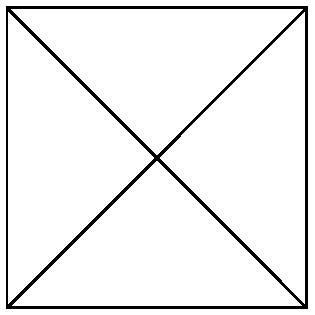
\includegraphics[scale=0.5]{figures/pyramid_tree_partition.pdf}
			}
			\end{subfloat}~
			\begin{subfloat}[Segmented $2d$ Pyramids, Each Associated with a Bucket\label{fig:pyramid-tree-buckets}] {%
				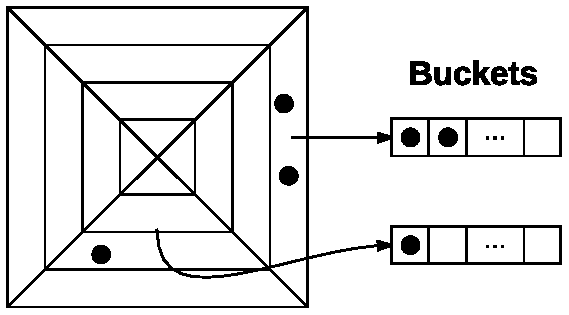
\includegraphics[scale=0.5]{figures/pyramid_tree_buckets.pdf}
			}
			\end{subfloat}
		\end{center}

		\label{fig:pyramid-tree-partition}
\end{figure}

TODO: define pyramid value

TODO: explain how a structure like the bucket ppt tree will be used

\subsection{Simple Bucket Hashmap}

TODO: extreme form of minimising bucket size -- average size almost one!

\subsection{New Baseline: $kd$-Tree}

Since the Octree cannot be used with high-dimensional data, a new baseline for evaluation (other than Seuqential Scan) was desired. The $kd$-tree is a widely used structure for both low and high dimensional data. This structure is multi-dimensional binary tree, meaning it does not have the expontential memory requirements the Octree has. This is because it splits the data space in a single dimension per level of the tree (referred to as a \textit{cutting dimension}), instead of splitting by \textit{all} dimensions. $kd$-trees are typically used for \textit{approximate} queries in higher-dimensional space, as they tend to degenerate to Sequential Scan for exact range and nearest neighbour queries \cite{similarity-searching}.

There are many variants of $kd$-trees \cite{kd-tree, bkd-tree, kdb-tree}. The variant implemented for this project contains one point per node and cycles through each dimension when choosing deciding which cutting dimension to use for each level of the tree. If $n$ is a $kd$-tree node, $i$ is the cutting dimension on that node's level and $p$ is the point stored in this node, then:
\begin{enumerate}
	\item $\forall q$ stored in the \textbf{left} subtree rooted at $n$: $p_i > q_i$ 
	\item $\forall q$ stored in the \textbf{right} subtree rooted at $n$: $p_i \leq q_i$.
\end{enumerate}
When inserting or querying a point $p$, the tree is traversed top-down in a similar fashion to a standard binary tree, by comparing $p_i$ to $n_i$, where $n$ is the point stored in the current node and $i$ is the cutting dimension of the current level.

% TODO: pseudo-code for this???
The \texttt{remove} operation\footnote{Source of \texttt{remove} algorithm is: \url{https://www.cs.umd.edu/class/spring2008/cmsc420/L19.kd-trees.pdf‎}} is more involved because it has to maintain the $kd$-tree invariant. To remove a point $p$, first the node containing $p$ is found using the aforementioned top-down traversal approach. Let $n$ be this node and $i$ be the current level's cutting dimension. If $n$ is a leaf, then the node can simply be deleted. Otherwise, let $n_L$ and $n_R$ be the left and right children of $n$ respectively. If $n_R$ exists, a node $m$ containing a point with the \textit{minimum} value for dimension $i$ is found in the sub-tree rooted at $n_R$. The points stored in nodes $n$ and $m$ are swapped and \texttt{delete($p$)} is called recursively on the sub-tree rooted at $n_R$. If $n_R$ does not exist, node $m$ is found in the sub-tree rooted at $n_L$ instead. In this case, after \texttt{delete($p$)} has been recursively called on the sub-tree rooted at $n_L$, the $i$th value of all points stored in this sub-tree are greater than or equal to the $i$th value of the new point in $n$. Therefore, $n_L$ then becomes the \textit{right} child of $n$ to maintain the $kd$-tree invariant.

TODO: figures showing example kd-tree, one insert and one remove (3 figures)

\subsection{Performance Timings}

TODO: four structures
	Bucket Pseudo-Pyramid Tree
	Boundary Distance Hashing
	Pyramid Tree
	kd-tree
	Simple Hashing

TODO: refer to plots and justify why only there's only two here (rest are in appendices)

TODO: table

TODO: plot of insert() w/ skewed data
TODO: plot of delete() w/ rand uniform data

\subsection{Profiling Results}

TODO: CPU/heap profiling

\subsection{Summary}

TODO
